\documentclass[12pt,a4paper]{article}

% ── Codificación y lenguaje ──
\usepackage[utf8]{inputenc}
\usepackage[T1]{fontenc}
% babel removed (Spanish language pack not available)

% ── Diseño de página ──
\usepackage[margin=2.5cm, top=3cm, bottom=3cm]{geometry}
\usepackage{fancyhdr}
\usepackage{lastpage}

% ── Tipografía ──
% lmodern and microtype removed (not available)

% ── Colores y gráficos ──
\usepackage[dvipsnames,svgnames,x11names]{xcolor}
\usepackage{tikz}
\usetikzlibrary{arrows.meta, positioning, shapes.geometric, calc, fit, backgrounds}
\usepackage{graphicx}
\usepackage{float}

% ── Código fuente ──
\usepackage{listings}

% ── Tablas ──
\usepackage{array}
\usepackage{booktabs}
\usepackage{multirow}
\usepackage{longtable}
\usepackage{tabularx}
\usepackage{colortbl}

% ── Otros ──
\usepackage{hyperref}
\usepackage{enumitem}
\usepackage{amsmath}
\usepackage{amssymb}
\usepackage{parskip}
\usepackage{titlesec}

% ══════════════════════════════════════════════════
%  CONFIGURACIÓN DE COLORES
% ══════════════════════════════════════════════════
\definecolor{uvggreen}{RGB}{0,100,60}
\definecolor{uvggold}{RGB}{192,160,64}
\definecolor{darkblue}{RGB}{20,40,80}
\definecolor{codebg}{RGB}{248,248,252}
\definecolor{codeframe}{RGB}{180,180,200}
\definecolor{keywordcolor}{RGB}{0,80,160}
\definecolor{stringcolor}{RGB}{180,40,40}
\definecolor{commentcolor}{RGB}{80,140,80}
\definecolor{sectionblue}{RGB}{15,50,100}
\definecolor{lightgray}{RGB}{240,240,245}
\definecolor{accentred}{RGB}{180,30,30}

% ══════════════════════════════════════════════════
%  CONFIGURACIÓN DE LISTINGS
% ══════════════════════════════════════════════════
\lstdefinestyle{pythonstyle}{
    language=Python,
    backgroundcolor=\color{codebg},
    frame=single,
    rulecolor=\color{codeframe},
    basicstyle=\ttfamily\footnotesize,
    keywordstyle=\color{keywordcolor}\bfseries,
    stringstyle=\color{stringcolor},
    commentstyle=\color{commentcolor}\itshape,
    numberstyle=\tiny\color{gray},
    numbers=left,
    numbersep=8pt,
    breaklines=true,
    breakatwhitespace=false,
    tabsize=4,
    showstringspaces=false,
    xleftmargin=18pt,
    framexleftmargin=15pt,
    aboveskip=12pt,
    belowskip=8pt,
    captionpos=b,
    literate={á}{{\'a}}1 {é}{{\'e}}1 {í}{{\'i}}1 {ó}{{\'o}}1 {ú}{{\'u}}1
             {ñ}{{\~n}}1 {Ñ}{{\~N}}1 {ε}{{$\varepsilon$}}1,
}

\lstdefinestyle{yalexstyle}{
    backgroundcolor=\color{codebg},
    frame=single,
    rulecolor=\color{codeframe},
    basicstyle=\ttfamily\footnotesize,
    keywordstyle=\color{keywordcolor}\bfseries,
    stringstyle=\color{stringcolor},
    commentstyle=\color{commentcolor}\itshape,
    numbers=left,
    numbersep=8pt,
    breaklines=true,
    tabsize=4,
    showstringspaces=false,
    xleftmargin=18pt,
    framexleftmargin=15pt,
    aboveskip=12pt,
    belowskip=8pt,
    morekeywords={let, rule, return, skip, eof},
    morestring=[b]',
    morestring=[b]",
    morecomment=[s]{(*}{*)},
    literate={á}{{\'a}}1 {é}{{\'e}}1 {í}{{\'i}}1 {ó}{{\'o}}1 {ú}{{\'u}}1,
}

\lstset{style=pythonstyle}

% ══════════════════════════════════════════════════
%  CONFIGURACIÓN DE ENCABEZADOS
% ══════════════════════════════════════════════════
\pagestyle{fancy}
\fancyhf{}
\fancyhead[L]{\small\textcolor{uvggreen}{\textbf{Universidad del Valle de Guatemala}}}
\fancyhead[R]{\small\textcolor{gray}{Proyecto 01 -- Generador de Analizadores Léxicos}}
\fancyfoot[C]{\thepage\ / \pageref{LastPage}}
\fancyfoot[R]{\small\textcolor{gray}{DLP 2026-I}}
\renewcommand{\headrulewidth}{0.8pt}
\renewcommand{\footrulewidth}{0.4pt}
\renewcommand{\headrule}{\hbox to\headwidth{\color{uvggreen}\leaders\hrule height \headrulewidth\hfill}}

% ══════════════════════════════════════════════════
%  FORMATO DE SECCIONES
% ══════════════════════════════════════════════════
\titleformat{\section}
  {\Large\bfseries\color{sectionblue}}
  {\thesection.}{0.5em}{}
  [\vspace{-4pt}\textcolor{uvggreen}{\rule{\textwidth}{1pt}}]

\titleformat{\subsection}
  {\large\bfseries\color{darkblue}}
  {\thesubsection}{0.5em}{}

\titleformat{\subsubsection}
  {\normalsize\bfseries\color{darkblue}}
  {\thesubsubsection}{0.5em}{}

% ══════════════════════════════════════════════════
%  HYPERREF
% ══════════════════════════════════════════════════
\hypersetup{
    colorlinks=true,
    linkcolor=darkblue,
    urlcolor=uvggreen,
    citecolor=accentred,
    pdftitle={Proyecto 01 - Generador de Analizadores Léxicos},
    pdfauthor={Diego Lopez, Jennifer Toxcon, Roberto Barreda},
}

% ══════════════════════════════════════════════════
%  DOCUMENTO
% ══════════════════════════════════════════════════
\begin{document}

% ── PORTADA ──────────────────────────────────────
\begin{titlepage}

\begin{tikzpicture}[remember picture, overlay]
  % Fondo superior
  \fill[uvggreen] (current page.north west) rectangle ([yshift=-6cm]current page.north east);
  % Franja dorada
  \fill[uvggold] ([yshift=-6cm]current page.north west) rectangle ([yshift=-6.4cm]current page.north east);
  % Franja inferior
  \fill[darkblue] (current page.south west) rectangle ([yshift=2.5cm]current page.south east);
\end{tikzpicture}

\vspace*{0.7cm}
\begin{center}
  {\Huge\bfseries\textcolor{white}{Universidad del Valle}}\\[6pt]
  {\Huge\bfseries\textcolor{white}{de Guatemala}}\\[14pt]
  {\large\textcolor{White}{Facultad de Ingeniería}}\\[4pt]
  {\large\textcolor{black}{Facultad de Ingeniería}}\\[4pt]
  {\large\textcolor{black}{Ciencia de la Computación y Tecnologías de la Información}}\\[1pt]
  {\normalsize\textcolor{black}{Diseño de Lenguajes de Programación - Sección 10}}\\[4pt]
  {\normalsize\textcolor{black}{Catedrático: Carlos Valdez}}
\end{center}

\vspace{3.5cm}

\begin{center}
  {\fontsize{28}{34}\selectfont\bfseries\textcolor{sectionblue}{Proyecto 01}}\\[18pt]
  {\fontsize{20}{26}\selectfont\textcolor{darkblue}{Generador de Analizadores Léxicos}}\\[10pt]
  {\Large\textcolor{uvggreen}{Implementación basada en YALex}}
\end{center}

\vspace{3cm}

\begin{center}
  \renewcommand{\arraystretch}{1.4}
  \begin{tabular}{r l}
    \textcolor{darkblue}{\textbf{Diego Lopez}}      & \textcolor{gray}{\#23747} \\
    \textcolor{darkblue}{\textbf{Jennifer Toxcon}}   & \textcolor{gray}{\#21276} \\
    \textcolor{darkblue}{\textbf{Roberto Barreda}}   & \textcolor{gray}{\#23354} \\
  \end{tabular}
\end{center}

\vfill
\begin{tikzpicture}[remember picture, overlay]
  \node[anchor=south, yshift=0.8cm] at (current page.south) {
    \textcolor{white}{\small Guatemala, 24 de marzo de 2026}
  };
\end{tikzpicture}
\end{titlepage}

% ── ÍNDICE ───────────────────────────────────────
\newpage
\tableofcontents
\newpage

% ══════════════════════════════════════════════════
%  1. INTRODUCCIÓN
% ══════════════════════════════════════════════════
\section{Introducción}

El presente informe documenta el diseño, la implementación y los resultados obtenidos en el \textbf{Proyecto 01} del curso \emph{Diseño de Lenguajes de Programación} (CC3071). El objetivo central del proyecto consiste en la construcción de un \textbf{generador de analizadores léxicos} inspirado en la herramienta YALex (\emph{Yet Another Lex}), la cual toma como referencia la implementación de \texttt{ocamllex} para OCaml.

Un analizador léxico (o \emph{lexer}) es la primera fase de un compilador o intérprete: su responsabilidad es leer una secuencia de caracteres de entrada y producir una secuencia de \emph{tokens}, es decir, unidades léxicas con significado dentro de la gramática del lenguaje. La generación automática de estos analizadores a partir de especificaciones de expresiones regulares es un problema clásico en ciencia de la computación, que involucra la teoría de autómatas finitos y la minimización de estados.

El proyecto abarca desde el \emph{parsing} de archivos de especificación \texttt{.yal}, pasando por la normalización de expresiones regulares, la construcción directa de Autómatas Finitos Deterministas (AFD) mediante el método del árbol sintáctico, la minimización de estados mediante particiones, y finalmente la generación de código Python autosuficiente que implementa el lexer resultante.

\subsection{Objetivos}

\begin{itemize}[leftmargin=2em]
  \item Implementar la construcción directa de AFD a partir de expresiones regulares utilizando el método del árbol sintáctico aumentado, sin recurrir a librerías de expresiones regulares.
  \item Implementar el algoritmo de minimización de AFD por particiones sucesivas.
  \item Diseñar y construir un parser para archivos de especificación en formato YALex (\texttt{.yal}).
  \item Generar archivos Python autosuficientes que funcionen como analizadores léxicos independientes del generador.
  \item Proveer una interfaz gráfica web amigable y estética para la interacción con el sistema.
  \item Validar el correcto funcionamiento con archivos de prueba de complejidad baja, media y alta.
\end{itemize}

\subsection{Repositorio}

El código fuente completo del proyecto se encuentra disponible en el siguiente repositorio de GitHub:

\begin{center}
  \url{https://github.com/bar23354/PRY1-DPL.git}
\end{center}

% ══════════════════════════════════════════════════
%  2. MARCO TEÓRICO
% ══════════════════════════════════════════════════
\section{Marco Teórico}

\subsection{Expresiones Regulares}

Las expresiones regulares constituyen un formalismo para describir conjuntos de cadenas (lenguajes regulares). En el contexto de la generación de analizadores léxicos, cada token se define mediante una expresión regular que describe el conjunto de lexemas válidos. Los operadores fundamentales son:

\begin{itemize}[leftmargin=2em]
  \item \textbf{Unión} (\texttt{|}): denota la alternativa entre dos expresiones.
  \item \textbf{Concatenación} (implícita): la yuxtaposición de dos expresiones.
  \item \textbf{Cerradura de Kleene} (\texttt{*}): cero o más repeticiones.
  \item \textbf{Cerradura positiva} (\texttt{+}): una o más repeticiones.
  \item \textbf{Opcionalidad} (\texttt{?}): cero o una ocurrencia.
\end{itemize}

La precedencia adoptada en YALex es, de mayor a menor: diferencia de conjuntos (\texttt{\#}), operadores unarios (\texttt{*}, \texttt{+}, \texttt{?}), concatenación, y unión (\texttt|}). Adicionalmente, se soportan conjuntos de caracteres (\texttt{[...]}), conjuntos negados (\texttt{[\^{}...]}), literales con comillas simples y dobles, el comodín \texttt{\_} (cualquier carácter) y la palabra reservada \texttt{eof}.

\subsection{Autómatas Finitos Deterministas (AFD)}

Un AFD se define formalmente como una 5-tupla $M = (Q, \Sigma, \delta, q_0, F)$ donde:

\begin{itemize}[leftmargin=2em]
  \item $Q$ es un conjunto finito de estados.
  \item $\Sigma$ es el alfabeto de entrada.
  \item $\delta: Q \times \Sigma \rightarrow Q$ es la función de transición.
  \item $q_0 \in Q$ es el estado inicial.
  \item $F \subseteq Q$ es el conjunto de estados de aceptación.
\end{itemize}

\subsection{Construcción Directa de AFD (Método del Árbol Sintáctico)}

El método directo evita la construcción intermedia de un AFN y opera directamente sobre el árbol sintáctico de la expresión regular aumentada ($r\#$). Para cada nodo del árbol se calculan cuatro funciones:

\begin{enumerate}[leftmargin=2em]
  \item \textbf{anulable}($n$): indica si el subárbol puede generar la cadena vacía ($\varepsilon$).
  \item \textbf{primeraPos}($n$): conjunto de posiciones (hojas) que pueden ser el primer símbolo en una cadena generada por el subárbol.
  \item \textbf{últimaPos}($n$): conjunto de posiciones que pueden ser el último símbolo.
  \item \textbf{siguientePos}($p$): para una posición $p$, el conjunto de posiciones que pueden seguir inmediatamente a $p$ en alguna cadena del lenguaje.
\end{enumerate}

Con estas funciones, el AFD se construye donde cada estado es un subconjunto de posiciones del árbol, el estado inicial es primeraPos de la raíz, y las transiciones se determinan mediante siguientePos.

\subsection{Minimización de AFD}

El algoritmo de minimización por particiones (Hopcroft) agrupa los estados en clases de equivalencia. Dos estados son equivalentes si, para cada símbolo del alfabeto, sus transiciones conducen a estados en la misma partición. El proceso itera hasta alcanzar un punto fijo donde ninguna partición puede refinarse más, produciendo el AFD mínimo equivalente.

\subsection{YALex: Especificación del Generador}

YALex (\emph{Yet Another Lex}) define un formato de archivo \texttt{.yal} con la siguiente estructura:

\begin{lstlisting}[style=yalexstyle, title={\small Estructura de un archivo YALex}]
{ header }
let ident = regexp
...
rule entrypoint [arg1, ..., argn] =
    regexp { action }
  | regexp { action }
  | ...
{ trailer }
\end{lstlisting}

Las secciones \texttt{header} y \texttt{trailer} son opcionales y se copian al inicio y final del archivo generado. Las definiciones \texttt{let} permiten nombrar expresiones regulares frecuentes. La sección \texttt{rule} define los patrones léxicos y sus acciones asociadas.

La política de matching es \emph{longest match}: se busca siempre el lexema más largo que haga concordancia; en caso de empate, se prioriza por orden de definición de las reglas.

% ══════════════════════════════════════════════════
%  3. ARQUITECTURA DEL SISTEMA
% ══════════════════════════════════════════════════
\section{Arquitectura del Sistema}

El sistema se organiza en una cadena de procesamiento (\emph{pipeline}) compuesta por módulos con responsabilidades bien definidas. La siguiente figura ilustra el flujo general:

\begin{figure}[H]
\centering
\resizebox{\textwidth}{!}{
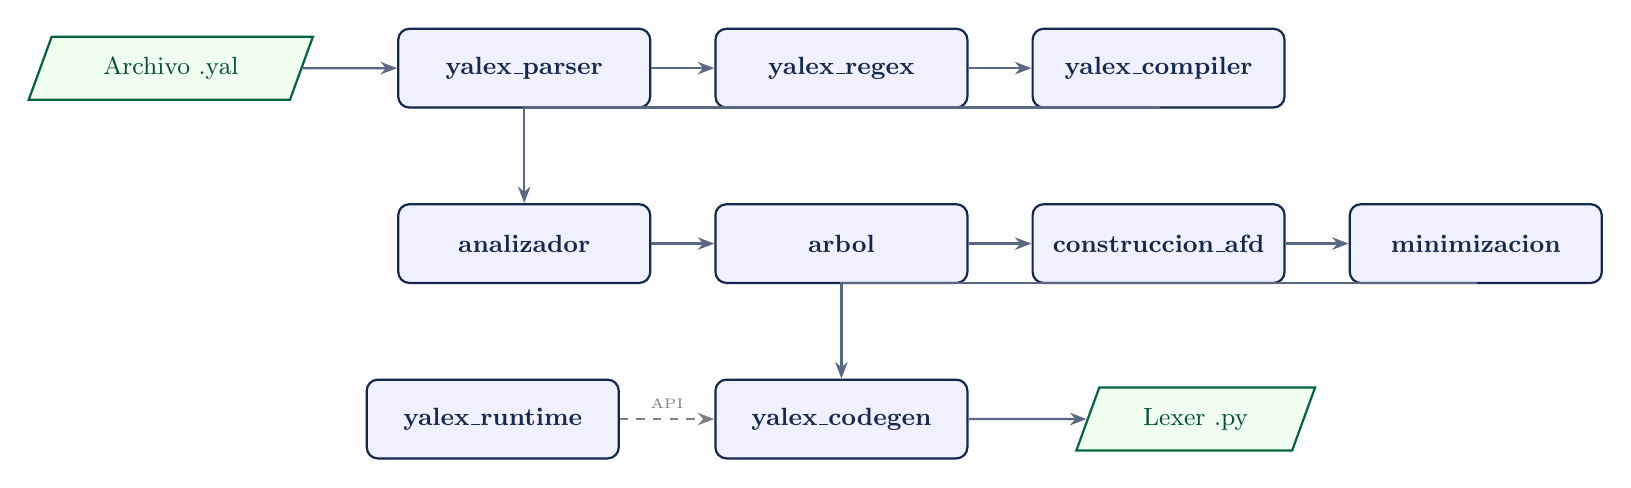
\begin{tikzpicture}[
    node distance=0.9cm and 0.4cm,
    box/.style={
        rectangle, rounded corners=4pt,
        draw=darkblue, thick,
        fill=blue!6,
        minimum width=3.2cm, minimum height=1cm,
        text centered, font=\small\bfseries,
        text=darkblue
    },
    io/.style={
        trapezium, trapezium left angle=70, trapezium right angle=110,
        draw=uvggreen, thick, fill=green!6,
        minimum width=2.4cm, minimum height=0.8cm,
        text centered, font=\small,
        text=uvggreen!80!black
    },
    arr/.style={-{Stealth[length=6pt]}, thick, color=darkblue!70},
]

% Fila superior: Entrada
\node[io] (yalin) {Archivo .yal};
\node[box, right=1.2cm of yalin] (parser) {yalex\_parser};
\node[box, right=0.8cm of parser] (regex) {yalex\_regex};
\node[box, right=0.8cm of regex] (compiler) {yalex\_compiler};

% Fila media: Pipeline interno
\node[box, below=1.2cm of parser] (analizador) {analizador};
\node[box, right=0.8cm of analizador] (arbol) {arbol};
\node[box, right=0.8cm of arbol] (afdmod) {construccion\_afd};
\node[box, right=0.8cm of afdmod] (minim) {minimizacion};

% Fila inferior: Salida
\node[box, below=1.2cm of arbol] (codegen) {yalex\_codegen};
\node[io, right=1.5cm of codegen] (salida) {Lexer .py};
\node[box, left=1.2cm of codegen] (runtime) {yalex\_runtime};

% Flechas superiores
\draw[arr] (yalin) -- (parser);
\draw[arr] (parser) -- (regex);
\draw[arr] (regex) -- (compiler);

% Flechas verticales
\draw[arr] (compiler) -- ++(0,-0.5) -| (analizador);
\draw[arr] (analizador) -- (arbol);
\draw[arr] (arbol) -- (afdmod);
\draw[arr] (afdmod) -- (minim);

% Flechas a salida
\draw[arr] (minim) -- ++(0,-0.5) -| (codegen);
\draw[arr] (codegen) -- (salida);

% Runtime
\draw[arr, dashed, color=gray] (runtime) -- (codegen) node[midway,above,font=\tiny\color{gray}] {API};

\end{tikzpicture}
}
\caption{Pipeline de compilación del generador YALex.}
\label{fig:pipeline}
\end{figure}

\subsection{Descripción de Módulos}

\begin{longtable}{>{\bfseries\ttfamily\small}p{3.8cm} p{10cm}}
\toprule
\normalfont\textbf{Módulo} & \textbf{Responsabilidad} \\
\midrule
\endhead
tokens.py & Define la representación interna de tokens (\texttt{Token} dataclass) con tipos literal, operador, épsilon y marcador. Incluye funciones auxiliares para clasificación y formateo de tokens. \\[6pt]
analizador.py & Tokenización de expresiones regulares, validación sintáctica, inserción explícita del operador de concatenación (\texttt{.}) y conversión a notación postfija mediante el algoritmo Shunting-Yard. \\[6pt]
arbol.py & Construcción del árbol sintáctico a partir de la expresión en postfijo. Cálculo de las funciones \emph{anulable}, \emph{primeraPos}, \emph{últimaPos} y \emph{siguientePos}. \\[6pt]
construccion\_afd.py & Construcción directa del AFD a partir del árbol sintáctico aumentado, generando estados como conjuntos de posiciones. \\[6pt]
minimizacion.py & Minimización del AFD mediante el algoritmo de refinamiento de particiones, produciendo el autómata mínimo equivalente. \\[6pt]
simulador.py & Simulación del AFD sobre cadenas de entrada, retornando el resultado (aceptación/rechazo) y el recorrido de estados. \\[6pt]
yalex\_parser.py & Parser del formato \texttt{.yal}: extrae header, trailer, definiciones \texttt{let}, entrypoint, argumentos y reglas con sus acciones. \\[6pt]
yalex\_regex.py & Normalizador de expresiones regulares YALex a formato interno. Maneja conjuntos, rangos, negaciones, literales, strings, diferencia de conjuntos (\texttt{\#}), wildcard (\texttt{\_}) y resolución de identificadores \texttt{let}. \\[6pt]
yalex\_compiler.py & Orquestador central: conecta el parser, el normalizador de regex, el constructor de AFD y el minimizador para producir un \texttt{CompiledLexer}. \\[6pt]
yalex\_codegen.py & Generador de código: produce un archivo Python autosuficiente que contiene los AFDs serializados y toda la lógica de scanning necesaria, sin dependencias externas. \\[6pt]
yalex\_runtime.py & Motor de ejecución del lexer en tiempo de compilación (uso interno). Implementa \emph{longest match} con desempate por prioridad de regla. \\[6pt]
\bottomrule
\end{longtable}

% ══════════════════════════════════════════════════
%  4. IMPLEMENTACIÓN
% ══════════════════════════════════════════════════
\section{Implementación}

\subsection{Tokenización y Conversión a Postfijo}

El módulo \texttt{analizador.py} implementa el pipeline fundamental para procesar expresiones regulares. La función \texttt{tokenizar} transforma una cadena de texto en una lista de objetos \texttt{Token}, reconociendo literales (incluyendo escapes con \texttt{\textbackslash}), operadores (\texttt{|}, \texttt{*}, \texttt{+}, \texttt{?}, paréntesis) y el símbolo épsilon ($\varepsilon$).

La validación sintáctica (\texttt{validarTokens}) verifica el balance de paréntesis, la ausencia de grupos vacíos y la correcta colocación de operadores unarios y binarios. Posteriormente, \texttt{insertarConcat} introduce operadores explícitos de concatenación (\texttt{.}) entre tokens adyacentes que lo requieran.

Finalmente, \texttt{aPostfijo} emplea el algoritmo \emph{Shunting-Yard} de Dijkstra para convertir la expresión infija a notación postfija, respetando la precedencia: unión (\texttt{|}) con precedencia 1 y concatenación (\texttt{.}) con precedencia 2.

\begin{lstlisting}[style=pythonstyle, caption={Tabla de precedencia y conversión a postfijo (fragmento).}]
precedencia = {'|': 1, '.': 2}

def aPostfijo(toks):
    salida, pila = [], []
    for token in toks:
        if es_literal(token) or es_epsilon(token):
            salida.append(token)
        elif es_operador(token, '('):
            pila.append(token)
        elif es_operador(token, ')'):
            while pila and not es_operador(pila[-1], '('):
                salida.append(pila.pop())
            pila.pop()
        elif es_unario(token):
            salida.append(token)
        elif es_binario(token):
            while (pila and es_binario(pila[-1])
                   and precedencia[pila[-1].value]
                       >= precedencia[token.value]):
                salida.append(pila.pop())
            pila.append(token)
    while pila:
        salida.append(pila.pop())
    return salida
\end{lstlisting}

\subsection{Árbol Sintáctico y Funciones de Posición}

El módulo \texttt{arbol.py} construye el árbol sintáctico a partir de la expresión en postfijo. Cada nodo \texttt{Nodo} almacena su valor (token), hijos izquierdo y derecho, y las propiedades calculadas: \texttt{anulable}, \texttt{primeraPos}, \texttt{últimaPos} y \texttt{siguientePos}.

Las reglas de cálculo implementadas son:

\begin{table}[H]
\centering
\renewcommand{\arraystretch}{1.4}
\begin{tabularx}{\textwidth}{|c|X|X|X|}
\hline
\rowcolor{lightgray}
\textbf{Nodo} & \textbf{anulable} & \textbf{primeraPos} & \textbf{últimaPos} \\
\hline
Hoja ($\varepsilon$) & \texttt{true} & $\emptyset$ & $\emptyset$ \\
\hline
Hoja (literal $i$) & \texttt{false} & $\{i\}$ & $\{i\}$ \\
\hline
$c_1 | c_2$ & $n(c_1) \lor n(c_2)$ & $pp(c_1) \cup pp(c_2)$ & $up(c_1) \cup up(c_2)$ \\
\hline
$c_1 \cdot c_2$ & $n(c_1) \land n(c_2)$ & si $n(c_1)$: $pp(c_1) \cup pp(c_2)$; sino: $pp(c_1)$ & si $n(c_2)$: $up(c_1) \cup up(c_2)$; sino: $up(c_2)$ \\
\hline
$c^*$, $c?$ & \texttt{true} & $pp(c)$ & $up(c)$ \\
\hline
$c^+$ & $n(c)$ & $pp(c)$ & $up(c)$ \\
\hline
\end{tabularx}
\caption{Reglas de cálculo para las funciones del árbol sintáctico.}
\end{table}

El cálculo de \texttt{siguientePos} se realiza en un recorrido postorden: para un nodo de concatenación $c_1 \cdot c_2$, se agrega $\text{primeraPos}(c_2)$ al conjunto siguientePos de cada posición en $\text{últimaPos}(c_1)$. Para nodos con cerradura (\texttt{*} o \texttt{+}), se agrega $\text{primeraPos}(n)$ a siguientePos de cada posición en $\text{últimaPos}(n)$.

\subsection{Construcción Directa del AFD}

El módulo \texttt{construccion\_afd.py} implementa la construcción directa. El estado inicial es $\text{primeraPos}(\text{raíz})$. Para cada estado (conjunto de posiciones) y cada símbolo del alfabeto, se calcula el nuevo estado como la unión de siguientePos de las posiciones cuyo símbolo coincida. Los estados que contengan la posición del marcador $\#$ se designan como estados de aceptación.

\begin{lstlisting}[style=pythonstyle, caption={Construcción directa del AFD (fragmento central).}]
def construirAfd(raiz, hojas, alfabeto):
    idMarcador = next(hid for hid, hoja in hojas.items()
                      if es_marker(hoja.valor))
    inicial = frozenset(raiz.primeraPos)
    porProcesar = [inicial]
    trans, aceptacion = {}, set()

    while porProcesar:
        actual = porProcesar.pop(0)
        for symbol in alfabeto:
            nuevo = set()
            for pos in actual:
                hoja = hojas[pos]
                if es_literal(hoja.valor)
                   and hoja.valor.value == symbol:
                    nuevo |= hoja.siguientePos
            if nuevo:
                nuevoFs = frozenset(nuevo)
                # registrar estado y transicion...
\end{lstlisting}

\subsection{Minimización del AFD}

El módulo \texttt{minimizacion.py} implementa el algoritmo de refinamiento de particiones. El proceso inicia con dos particiones: estados de aceptación y estados de no-aceptación. En cada iteración, se calcula una ``firma'' para cada estado basada en las particiones a las que conducen sus transiciones. Los estados con firmas diferentes dentro de una misma partición se separan.

El proceso itera hasta que no se produzcan más cambios, generando el AFD mínimo con nomenclatura \texttt{M0}, \texttt{M1}, etc.

\subsection{Parser de Archivos YALex}

El módulo \texttt{yalex\_parser.py} implementa un parser completo para la especificación YALex. Las funcionalidades principales incluyen:

\begin{itemize}[leftmargin=2em]
  \item \textbf{Eliminación de comentarios}: soporte para delimitadores \texttt{(* ... *)}.
  \item \textbf{Extracción de header/trailer}: bloques opcionales delimitados por llaves.
  \item \textbf{Definiciones let}: parseo de \texttt{let ident = regexp} con validación de identificadores.
  \item \textbf{Cabecera de rule}: extracción del entrypoint y argumentos opcionales.
  \item \textbf{Reglas léxicas}: separación por \texttt{|} a nivel superior, identificación de patrones y acciones respetando niveles de anidamiento en paréntesis, corchetes, llaves y cadenas.
\end{itemize}

El parser produce un objeto \texttt{YalexSpec} que encapsula toda la información estructurada de la especificación.

\subsection{Normalizador de Expresiones Regulares YALex}

El módulo \texttt{yalex\_regex.py} convierte la sintaxis rica de YALex a la representación interna del motor de regex. Implementa un parser descendente recursivo con la siguiente jerarquía de precedencia:

\begin{enumerate}[leftmargin=2em]
  \item \texttt{\_parse\_union}: maneja alternativas (\texttt{|}).
  \item \texttt{\_parse\_concat}: maneja concatenación implícita.
  \item \texttt{\_parse\_unary}: maneja \texttt{*}, \texttt{+}, \texttt{?}.
  \item \texttt{\_parse\_difference}: maneja diferencia de conjuntos (\texttt{\#}).
  \item \texttt{\_parse\_atom}: maneja literales, strings, conjuntos, identificadores, paréntesis y \texttt{eof}.
\end{enumerate}

La resolución de identificadores \texttt{let} se realiza con detección de ciclos mediante una pila de nombres para prevenir referencias recursivas.

\subsection{Compilador y Generador de Código}

El módulo \texttt{yalex\_compiler.py} conecta todos los componentes anteriores. Para cada regla del archivo \texttt{.yal}, normaliza la expresión regular, construye el AFD directo y lo minimiza. El resultado es un \texttt{CompiledLexer} que contiene la lista de reglas compiladas con sus respectivos AFDs.

El módulo \texttt{yalex\_codegen.py} toma este \texttt{CompiledLexer} y genera un archivo Python completamente autosuficiente. El archivo generado incluye:

\begin{itemize}[leftmargin=2em]
  \item Los AFDs serializados como diccionarios Python.
  \item Clases \texttt{LexToken} y \texttt{YalexLexError}.
  \item La función \texttt{scan} con lógica de \emph{longest match} y desempate por prioridad.
  \item La función del entrypoint nombrada según la especificación.
  \item Las secciones de header y trailer copiadas literalmente.
\end{itemize}

Este diseño garantiza que el lexer generado no dependa del generador, cumpliendo el requisito de independencia establecido en la rúbrica.

\subsection{Motor de Ejecución (\emph{Runtime})}

El módulo \texttt{yalex\_runtime.py} implementa la lógica de scanning utilizada tanto internamente como la que se embebe en el código generado. La función \texttt{\_max\_prefix\_match} simula el AFD de cada regla para encontrar el prefijo más largo que sea aceptado. La función \texttt{scan} aplica la política de \emph{longest match}:

\begin{enumerate}[leftmargin=2em]
  \item Para cada posición en el texto, se prueban todas las reglas.
  \item Se selecciona la regla con el match más largo.
  \item En caso de empate en longitud, se prioriza la regla con menor índice (orden de definición).
  \item Se ejecuta la acción asociada. Si retorna \texttt{SKIP}, se avanza sin emitir token.
  \item El proceso continúa hasta consumir toda la entrada.
\end{enumerate}

% ══════════════════════════════════════════════════
%  5. RESTRICCIONES Y DECISIONES DE DISEÑO
% ══════════════════════════════════════════════════
\section{Restricciones y Decisiones de Diseño}

\subsection{Prohibición de Librerías de Regex}

Una restricción fundamental del proyecto es la prohibición total del uso de librerías de expresiones regulares (como el módulo \texttt{re} de Python). Todo el matching léxico se implementa mediante autómatas finitos construidos desde cero. El incumplimiento de esta restricción conlleva una calificación de 0 puntos.

La implementación respeta esta restricción en su totalidad: la tokenización se realiza carácter por carácter, la construcción de autómatas es directa, y la simulación opera sobre las tablas de transición generadas.

\subsection{Independencia del Lexer Generado}

El archivo Python generado por \texttt{yalex\_codegen.py} es completamente autosuficiente. No importa ningún módulo del paquete \texttt{laboratorio}, sino que incluye dentro de sí mismo todas las estructuras de datos necesarias (clases, funciones de matching, función scan) y los AFDs serializados como diccionarios nativos de Python.

\subsection{Interfaz Gráfica}

El proyecto incluye una interfaz web implementada en HTML, CSS y JavaScript puro, organizada en múltiples vistas especializadas. Esta interfaz permite interactuar con el generador de analizadores léxicos de manera visual e intuitiva, cumpliendo con el requisito de ser ``amigable y estética''.

% ══════════════════════════════════════════════════
%  6. ARCHIVOS DE PRUEBA
% ══════════════════════════════════════════════════
\section{Archivos de Prueba}

Se desarrollaron tres pares de archivos de prueba con complejidades crecientes, almacenados en la carpeta \texttt{examples/} del repositorio.

\subsection{Complejidad Baja}

La especificación de complejidad baja reconoce tokens aritméticos básicos: identificadores, números enteros (incluyendo negativos), operadores aritméticos y de asignación, y espacios en blanco (que se omiten).

\begin{lstlisting}[style=yalexstyle, caption={Ejemplo de entrada de complejidad baja.}]
variable + 5 * -11 = otraVariable
\end{lstlisting}

Tokens esperados: \texttt{ID}, \texttt{PLUS}, \texttt{NUMBER}, \texttt{TIMES}, \texttt{NUMBER}, \texttt{ASSIGN}, \texttt{ID}.

\subsection{Complejidad Media}

La especificación de complejidad media incorpora palabras reservadas (\texttt{if}, \texttt{else}, \texttt{while}), operadores de comparación (\texttt{>=}, \texttt{==}), cadenas entre comillas y una variedad más amplia de tokens.

\begin{lstlisting}[style=yalexstyle, caption={Ejemplo de entrada de complejidad media.}]
if x1 >= 10 else while nombre == "abc"
\end{lstlisting}

\subsection{Complejidad Alta}

La especificación de complejidad alta simula un subconjunto de un lenguaje tipo C, con tipos de datos (\texttt{int}, \texttt{float}), literales de punto flotante, operadores lógicos (\texttt{\&\&}, \texttt{||}), operadores de comparación compuestos (\texttt{<=}, \texttt{!=}), delimitadores de bloque, punto y coma, y la palabra reservada \texttt{return}.

\begin{lstlisting}[style=yalexstyle, caption={Ejemplo de entrada de complejidad alta.}]
int x = 10;
float y = 20.5;
if (x <= y && x != 0) { return x; }
\end{lstlisting}

% ══════════════════════════════════════════════════
%  7. PRUEBAS Y RESULTADOS
% ══════════════════════════════════════════════════
\section{Pruebas y Resultados}

El proyecto cuenta con una suite de pruebas automatizadas exhaustiva implementada con \texttt{pytest}. Las pruebas cubren todos los criterios de la rúbrica de evaluación.

\subsection{Estructura de la Suite de Pruebas}

\begin{table}[H]
\centering
\renewcommand{\arraystretch}{1.3}
\begin{tabularx}{\textwidth}{>{\ttfamily\small}l X}
\toprule
\normalfont\textbf{Archivo de prueba} & \textbf{Cobertura} \\
\midrule
test\_analizador.py & Tokenización, validación, inserción de concatenación y conversión a postfijo. \\
test\_arbol\_y\_afd.py & Construcción del árbol sintáctico y generación directa de AFD. \\
test\_minimizacion.py & Algoritmo de minimización y métricas comparativas. \\
test\_integracion.py & Flujos completos de regex a AFD minimizado. \\
test\_yalex\_parser.py & Parsing de archivos \texttt{.yal} con todas sus variantes. \\
test\_yalex\_codegen.py & Generación de código autosuficiente y su correcta ejecución. \\
test\_yalex\_runtime.py & Motor de ejecución con \emph{longest match} y manejo de errores. \\
test\_yalex\_spec\_completo.py & Especificaciones YALex completas de extremo a extremo. \\
test\_rubrica\_proyecto01.py & Pruebas alineadas exactamente con la rúbrica de evaluación. \\
\bottomrule
\end{tabularx}
\caption{Archivos de prueba y su cobertura funcional.}
\end{table}

\subsection{Cumplimiento de la Rúbrica}

La siguiente tabla detalla el cumplimiento de cada criterio de la rúbrica, incluyendo el test específico que lo valida:

\begin{longtable}{p{7.5cm} c p{4.8cm}}
\toprule
\textbf{Criterio} & \textbf{Pts} & \textbf{Test de validación} \\
\midrule
\endhead
Generación de diagrama de transición de estados & 1 & \texttt{test\_diagrama\_transicion} \\[4pt]
Baja: identificación de tokens & 0.5 & \texttt{test\_baja\_identifica\_tokens} \\[4pt]
Baja: detección de errores & 0.5 & \texttt{test\_baja\_detecta\_error} \\[4pt]
Baja modificada: ident. de tokens & 0.5 & \texttt{test\_baja\_mod\_identifica} \\[4pt]
Baja modificada: detección de errores & 0.5 & \texttt{test\_baja\_mod\_detecta\_error} \\[4pt]
Media: identificación de tokens & 1 & \texttt{test\_media\_identifica\_tokens} \\[4pt]
Media: detección de errores & 1 & \texttt{test\_media\_detecta\_error} \\[4pt]
Media modificada: ident. de tokens & 1 & \texttt{test\_media\_mod\_identifica} \\[4pt]
Media modificada: detección de errores & 1 & \texttt{test\_media\_mod\_detecta\_error} \\[4pt]
Alta: identificación de tokens & 1.5 & \texttt{test\_alta\_identifica\_tokens} \\[4pt]
Alta: detección de errores & 1.5 & \texttt{test\_alta\_detecta\_error} \\[4pt]
Alta modificada: ident. de tokens & 2 & \texttt{test\_alta\_mod\_identifica} \\[4pt]
Alta modificada: detección de errores & 2 & \texttt{test\_alta\_mod\_detecta\_error} \\[4pt]
\midrule
\textbf{Subtotal funcionalidad} & \textbf{14} & \\
Preguntas orales (2 por estudiante) & 6 & Evaluación presencial \\
\midrule
\textbf{Total} & \textbf{20} & \\
\bottomrule
\end{longtable}

\subsection{Penalizaciones Evitadas}

\begin{table}[H]
\centering
\renewcommand{\arraystretch}{1.3}
\begin{tabularx}{\textwidth}{X c l}
\toprule
\textbf{Restricción} & \textbf{Penalización} & \textbf{Estado} \\
\midrule
Interfaz gráfica amigable y estética & $-3$ pts & \textcolor{uvggreen}{\textbf{Cumplido}} \\
Lexer generado independiente del generador & $-3$ pts & \textcolor{uvggreen}{\textbf{Cumplido}} \\
No usar librerías de regex & $= 0$ pts & \textcolor{uvggreen}{\textbf{Cumplido}} \\
Archivos de prueba baja/media/alta & $= 0$ pts & \textcolor{uvggreen}{\textbf{Cumplido}} \\
\bottomrule
\end{tabularx}
\caption{Restricciones y estado de cumplimiento.}
\end{table}

% ══════════════════════════════════════════════════
%  8. FLUJO DE EJECUCIÓN
% ══════════════════════════════════════════════════
\section{Flujo de Ejecución}

El sistema ofrece dos modos de operación principales:

\subsection{Modo Consola (Expresiones Regulares)}

Mediante \texttt{python main.py}, el usuario puede:
\begin{enumerate}[leftmargin=2em]
  \item Ingresar una expresión regular arbitraria.
  \item Visualizar la expresión con concatenación explícita y en notación postfija.
  \item Inspeccionar el AFD directo y el AFD minimizado (tablas de transición).
  \item Comparar métricas entre ambos autómatas.
  \item Validar cadenas contra el AFD minimizado.
\end{enumerate}

\subsection{Modo Generador YALex (CLI)}

Mediante \texttt{python yalex.py archivo.yal -o nombre\_salida}, el sistema:
\begin{enumerate}[leftmargin=2em]
  \item Lee y parsea el archivo \texttt{.yal}.
  \item Normaliza cada expresión regular de las reglas.
  \item Construye y minimiza un AFD por cada regla.
  \item Genera un archivo Python autosuficiente con el lexer.
  \item Reporta el número de reglas compiladas y la presencia de header/trailer.
\end{enumerate}

El archivo generado puede utilizarse directamente:

\begin{lstlisting}[style=pythonstyle, caption={Uso del lexer generado.}]
# Importar el lexer generado
from thelexer import gettoken  # nombre del entrypoint

# Tokenizar una entrada
tokens = gettoken("int x = 42;")
for tok in tokens:
    print(f"{tok.type}: {tok.lexeme!r}")
\end{lstlisting}

% ══════════════════════════════════════════════════
%  9. DIAGRAMA DE CLASES Y ESTRUCTURAS
% ══════════════════════════════════════════════════
\section{Estructuras de Datos Principales}

\begin{figure}[H]
\centering
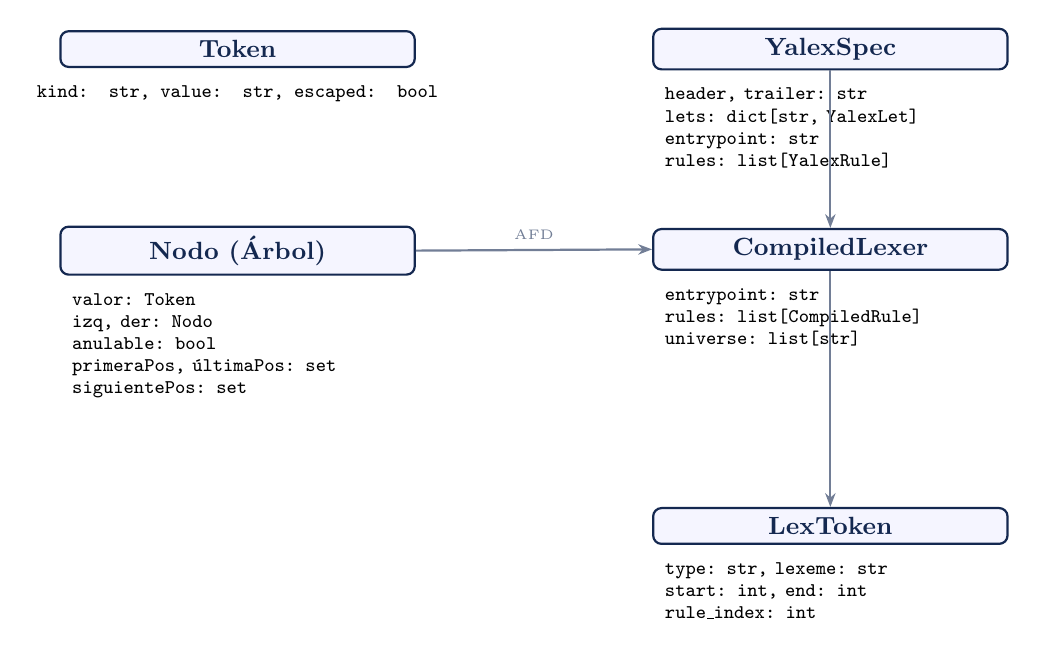
\begin{tikzpicture}[
    class/.style={
        rectangle, draw=darkblue, thick, rounded corners=3pt,
        fill=blue!4, text=darkblue,
        minimum width=4.5cm,
        font=\small
    },
    field/.style={font=\ttfamily\scriptsize, text=black},
    arr/.style={-{Stealth[length=5pt]}, thick, darkblue!60},
    node distance=0.6cm
]

% Token
\node[class] (token) {\textbf{Token}};
\node[field, below=0.1cm of token] (tf) {kind: str, value: str, escaped: bool};

% YalexSpec
\node[class, right=3cm of token] (spec) {\textbf{YalexSpec}};
\node[field, below=0.1cm of spec, text width=4.2cm, align=left] (sf) {header, trailer: str\\lets: dict[str, YalexLet]\\entrypoint: str\\rules: list[YalexRule]};

% Nodo
\node[class, below=2cm of token] (nodo) {\textbf{Nodo (Árbol)}};
\node[field, below=0.1cm of nodo, text width=4.2cm, align=left] (nf) {valor: Token\\izq, der: Nodo\\anulable: bool\\primeraPos, últimaPos: set\\siguientePos: set};

% CompiledLexer
\node[class, below=2cm of spec] (compiled) {\textbf{CompiledLexer}};
\node[field, below=0.1cm of compiled, text width=4.2cm, align=left] (cf) {entrypoint: str\\rules: list[CompiledRule]\\universe: list[str]};

% LexToken
\node[class, below=3cm of compiled] (lextoken) {\textbf{LexToken}};
\node[field, below=0.1cm of lextoken, text width=4.2cm, align=left] (lf) {type: str, lexeme: str\\start: int, end: int\\rule\_index: int};

% Arrows
\draw[arr] (spec.south) -- (compiled.north);
\draw[arr] (nodo.east) -- (compiled.west) node[midway, above, font=\tiny] {AFD};
\draw[arr] (compiled.south) -- (lextoken.north);

\end{tikzpicture}
\caption{Estructuras de datos principales del sistema.}
\label{fig:clases}
\end{figure}

% ══════════════════════════════════════════════════
%  10. CUMPLIMIENTO DE CONSIDERACIONES YALEX
% ══════════════════════════════════════════════════
\section{Cumplimiento de Consideraciones YALex}

La siguiente tabla resume el cumplimiento de cada aspecto de las consideraciones YALex proporcionadas en el enunciado del proyecto:

\begin{longtable}{p{6.5cm} c p{5.5cm}}
\toprule
\textbf{Consideración} & \textbf{Estado} & \textbf{Implementación} \\
\midrule
\endhead
Estructura del archivo \texttt{.yal} & \textcolor{uvggreen}{\checkmark} & \texttt{yalex\_parser.py} \\[4pt]
Header y trailer opcionales & \textcolor{uvggreen}{\checkmark} & Extracción por llaves \\[4pt]
Definiciones \texttt{let ident = regexp} & \textcolor{uvggreen}{\checkmark} & Resolución recursiva con detección de ciclos \\[4pt]
Comentarios \texttt{(* ... *)} & \textcolor{uvggreen}{\checkmark} & \texttt{\_strip\_comments} \\[4pt]
Literales de carácter (\texttt{'c'}) & \textcolor{uvggreen}{\checkmark} & \texttt{\_read\_quoted\_char} \\[4pt]
Constantes tipo cadena (\texttt{"str"}) & \textcolor{uvggreen}{\checkmark} & \texttt{\_read\_quoted\_string} \\[4pt]
Conjuntos \texttt{[...]} & \textcolor{uvggreen}{\checkmark} & \texttt{\_set\_to\_expr} \\[4pt]
Conjuntos negados \texttt{[\^{}...]} & \textcolor{uvggreen}{\checkmark} & Complemento sobre universo \\[4pt]
Rangos \texttt{'a'-'z'} & \textcolor{uvggreen}{\checkmark} & \texttt{\_parse\_set\_item} \\[4pt]
Diferencia de conjuntos (\texttt{\#}) & \textcolor{uvggreen}{\checkmark} & \texttt{\_parse\_difference} \\[4pt]
Wildcard (\texttt{\_}) & \textcolor{uvggreen}{\checkmark} & Expansión a todo el universo \\[4pt]
Cerradura \texttt{*}, \texttt{+}, \texttt{?} & \textcolor{uvggreen}{\checkmark} & \texttt{\_parse\_unary} \\[4pt]
Concatenación y unión & \textcolor{uvggreen}{\checkmark} & Parser descendente recursivo \\[4pt]
Identificador \texttt{eof} & \textcolor{uvggreen}{\checkmark} & Manejo especial en \texttt{\_parse\_atom} \\[4pt]
Secuencias de escape & \textcolor{uvggreen}{\checkmark} & \texttt{\_decode\_escape} \\[4pt]
Longest match & \textcolor{uvggreen}{\checkmark} & \texttt{\_max\_prefix\_match} \\[4pt]
Desempate por orden de regla & \textcolor{uvggreen}{\checkmark} & Comparación por \texttt{rule.index} \\[4pt]
Acciones con \texttt{return} y \texttt{skip} & \textcolor{uvggreen}{\checkmark} & \texttt{\_build\_action\_callable} \\[4pt]
\bottomrule
\end{longtable}

% ══════════════════════════════════════════════════
%  11. EJEMPLO DE EJECUCIÓN COMPLETA
% ══════════════════════════════════════════════════
\section{Ejemplo de Ejecución Completa}

A continuación se ilustra el flujo completo para la expresión regular \texttt{(a|b)*abb}:

\begin{enumerate}[leftmargin=2em]
  \item \textbf{Tokenización}: Se produce la lista de tokens: \texttt{(}, \texttt{a}, \texttt{|}, \texttt{b}, \texttt{)}, \texttt{*}, \texttt{a}, \texttt{b}, \texttt{b}.

  \item \textbf{Inserción de concatenación}: Se insertan operadores explícitos: \texttt{(a|b)*}\textbf{.}\texttt{a}\textbf{.}\texttt{b}\textbf{.}\texttt{b}.

  \item \textbf{Postfijo}: La conversión produce: \texttt{a b | * a . b . b .}

  \item \textbf{Árbol sintáctico aumentado}: Se agrega el marcador \texttt{\#} y se construye el árbol con las funciones de posición calculadas en cada nodo.

  \item \textbf{Construcción del AFD}: Se genera el AFD directo con estados como conjuntos de posiciones de las hojas del árbol.

  \item \textbf{Minimización}: Se aplica el algoritmo de particiones para obtener el AFD mínimo equivalente.
\end{enumerate}

% ══════════════════════════════════════════════════
%  12. CONCLUSIONES
% ══════════════════════════════════════════════════
\section{Conclusiones}

\begin{enumerate}[leftmargin=2em]
  \item Se implementó exitosamente un generador de analizadores léxicos basado en la especificación YALex, cubriendo todos los aspectos funcionales requeridos por la rúbrica del proyecto.

  \item La construcción directa de AFD mediante el método del árbol sintáctico demostró ser una alternativa eficiente a la construcción vía AFN-$\varepsilon$, eliminando la necesidad de la conversión de subconjuntos y produciendo directamente un autómata determinista.

  \item El algoritmo de minimización por particiones reduce de manera efectiva el número de estados, optimizando tanto el uso de memoria como el rendimiento del lexer generado durante la fase de scanning.

  \item La arquitectura modular del sistema, con separación clara entre parsing, normalización, construcción de autómatas, minimización y generación de código, facilita el mantenimiento, la depuración y la extensión futura del proyecto.

  \item La generación de código autosuficiente garantiza que los analizadores léxicos producidos sean portables y no dependan del entorno del generador, lo cual es fundamental para su integración en cadenas de compilación reales.

  \item La implementación completa sin librerías de expresiones regulares demuestra la comprensión profunda de la teoría de autómatas finitos y su aplicación práctica en el diseño de lenguajes de programación.

  \item La suite de pruebas automatizadas proporciona una validación rigurosa del sistema, cubriendo los tres niveles de complejidad (baja, media y alta) tanto en su forma original como modificada.
\end{enumerate}

% ══════════════════════════════════════════════════
%  13. REFERENCIAS
% ══════════════════════════════════════════════════
\section{Referencias}

\begin{enumerate}[leftmargin=2em, label={[\arabic*]}]
  \item Aho, A. V., Lam, M. S., Sethi, R., \& Ullman, J. D. (2006). \emph{Compilers: Principles, Techniques, and Tools} (2nd ed.). Addison-Wesley.
  \item Hopcroft, J. E., Motwani, R., \& Ullman, J. D. (2006). \emph{Introduction to Automata Theory, Languages, and Computation} (3rd ed.). Pearson.
  \item Leroy, X. et al. \emph{The OCaml system: Documentation and user's manual}. Capítulo sobre ocamllex.
  \item Valdez, C. (2026). \emph{Consideraciones de YALex}. Universidad del Valle de Guatemala, CC3071.
  \item Valdez, C. (2026). \emph{Proyecto 01 -- Rúbrica de evaluación}. Universidad del Valle de Guatemala, CC3071.
\end{enumerate}

\end{document}
